\documentclass{article}
\usepackage[utf8]{inputenc}

\title{Variable Intake Electronics Subsystem}
\author{John Wiggins }
\date{December 2019}

\usepackage{natbib}
\usepackage{graphicx}

\begin{document}

\maketitle

\section{Introduction}
The goals of this project were to develop a lightweight electronics housing system that could communicate via CAN bus. The RPM of the AR 20 vehicle would be then logged onto a microprocessor and converted to length, via the Helmholtz relationship between length and RPM.


\begin{figure}[h!]
\centering
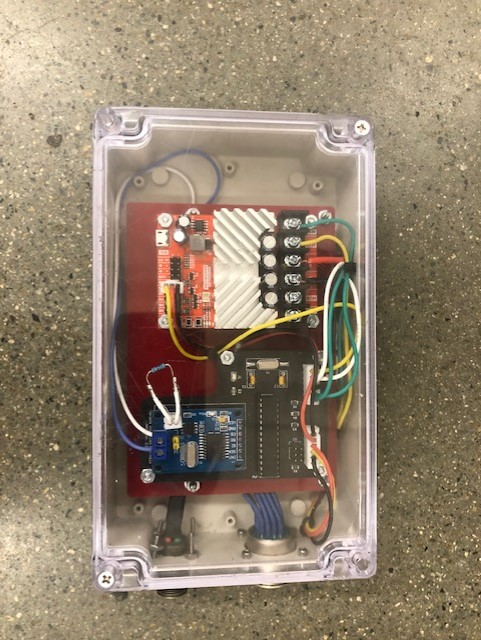
\includegraphics[scale=0.5, angle = 90]{Electronics_Housing.jpg}
\caption{Electronics Housing Assembly}
\label{fig:assembly}
\end{figure}

\section{Components}
This project was split into two major subsystems. The first subsystem is the On-Board controller housing that lives in the Side-Pod. The second subsystem is the Simulated Interactive Display (SID) that allowed for tuning of the electronics system without the car running.
\subsection{On-Board systems}
The on-board system has two main components: The roboclaw motor controller and the custom CAN to SPI conversion Micro-Controller, known as CAN Variable Actuation System (CANVAS).

\subsubsection{RoboCLaw}
The RoboClaw motor controller controls the actuator's DC motor via a PWM signal from the CANVAS board. 
\newline 
\begin{figure}[h!]
\centering
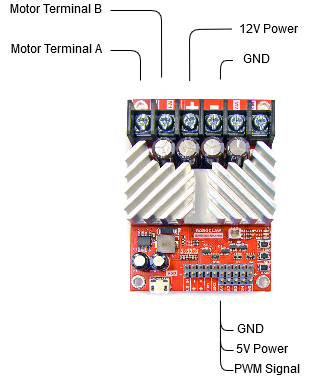
\includegraphics[scale=0.6]{ME_490_Drawings.png}
\caption{RoboClaw Project Wiring Diagram}
\label{fig:roboclaw}
\end{figure}

These are a few notes about the modes and operation of the RoboClaw:
\begin{itemize}
    \item The board is set to be in ANALOG MODE 3 for PWM interpretation.
    \item The board regulates the power for the CANVAS board down to 5V which is is the primary source of power for the board. It saved the project having to add an external voltage regulator or separate power source for the CANVAS board.
    \item The rapid indicator flashing notes that it is receiving signals.
    \item Do not attempt to use serial for communication with the RoboClaw for this project. There was success using serial, however, the CANVAS board was having trouble with dual serial communications and worked more reliably using PWM.
\end{itemize}

\subsubsection{CANVAS PCB}
The CANVAS PCB operates as the MCU for the on-board system. With an integrated CAN Bus converter, the board operates as the interface between the vehicle and the motor controller. For more information on the board, refer to the CANVAS PCB Design section. 

\section{CANVAS PCB Design}
\section{CAN Communication Notes}
\section{Static Interactive Display (SID)}
\section{Vehicle Constraints}
\section{Manufacturing}
\section{Safety}

\section{Operation}
In order to operate the system safely, please follow these steps on powering up, powering down, and controlling the system.
\subsection{Powering Up}
\subsubsection{Normal Driving Operation (NDO)}
Normal Driving Operation (NDO) is used when vehicle is to be driven around.
\begin{enumerate}
    \item Verify all connections are secure on the vehicle (Under-Dash CAN, Actuator Clip, and Side-Pod Terminals).
    \item Turn the power safety clip on the drivers right hand side of the vehicle to the ON position.
    \item Wait for power on sequence. (NOTE: Actuator will move to lowest position).
    \item System is ready to drive.
\end{enumerate}
\subsubsection{Bench Power and Simulated RPM}
Bench Power is for when the vehicle is static and power does not want to be drained from on-board battery. To move actuator, use of the SID will be needed.
\begin{enumerate}
    \item Lift and secure Side-Pod on the side of the vehicle.
    \item Remove screws from top acrylic cover of actuator casing.
    \item Remove the 2-Prong Power connectors to the vehicle on the lower left side of the casing. This keeps the rest of the vehicle from getting power and turning on the built in CAN bus system from the Motec ECU.
    \item Verify bench power supply is \textit{NOT} connected to the vehicle.
    \item Turn ON bench power supply and verify the output voltage is set to 12V.
    \item Turn OFF bench power supply.
    \item Reach under dash and disconnect CAN bus terminals.
    \item Connect the CAN bus terminal going to the sidepod to the SID CAN bus line.
    \item Connect the power and ground terminals of the Roboclaw to the bench power supply.
    \item Connect the SID to power via Mini USB.
    \item Power on bench power supply.
    \item Wait for startup sequence.
    \item System is ready to simulate.
\end{enumerate}

\subsection{Powering Down}
\subsubsection{Normal Driving Operation (NDO)}
To power down, turning off power to the vehicle will shutdown the system immediately. 
\newline \newline 
NOTE: If the operator wishes the actuator to go to the fully contracted position, power cycling the car will trigger the boot up sequence, which sets the actuator to the fully contracted position. Do NOT turn the vehicle back on once it is in this position as it will move the actuator automatically to the the optimized intake length for the given RPM.

\subsubsection{Bench Power and Simulated RPM}
\begin{enumerate}
    \item Move the actuator to the fully contracted position, for storage and quality maintenance of actuator.
    \item Power off the bench power supply. This guarantees the actuator is no longer able to move.
    \item Power off the SID.
    \item Reconnect the dash CAN bus clip to the built in vehicle terminal.
    \item Reconnect the Side-Pod housing to the built in vehicle power terminals.
    \item Verify all connections are restored for driving operation and close and secure Side-Pod.
\end{enumerate}

\subsection{Control via Static Interface Display (SID)}
For operating the SID, please follow these steps.
\subsubsection{Boot Up Sequence}
The SID has a boot up sequence that initialized the CAN bus inside the box. When the boot is set, the LCD monitor will display that the CAN bus has been initialized. Press the MODE button to move into the operating modes. The indicator LED will begin to glow to reflect the current user mode.
\subsubsection{RPM Tuning}
The RPM Tuning mode is controlled by the potentiometer in the middle of the base panel. The RPM is displayed on the LCD as well as the intended length and position of the actuator. This mode will run until the MODE button is pressed, indicating the mode to jump out of it's loop and upon a second press of the MODE button, will move onto the next MODE of operation.
\subsubsection{Fully Extended}
Fully Extended mode moves the actuator to the longest length the on-board Side-Pod housing controller allows. Upon arrival at this location, the user can press MODE again to jump out of the movement of the actuation and upon a secondary press, can change to the next MODE.
\newline \newline
NOTE: Do NOT click the MODE button while the actuator is moving. This will lock the movement of the actuator causing it to over extend and could damage the machine. Currently working on fixes for this issue, however for the time-being, please be aware of this and use with caution.
\subsubsection{Fully Contracted}
Fully Contracted mode move the actuator to the shortest length the on-board Side-Pod housing controller allows. Upon arrival at this location, the user can press MODE again to jump out of the movement of the actuation and upon a secondary press, can change to the next MODE.
\subsubsection{Range of Actuation Demo}
The Range of Actuation Demo allows for the demonstration of the continuous range of motion the actuator allows. This mode will toggle between fully extended and fully contracted.
\newline \newline
NOTE: To move on from this mode, hold the MODE button down until the actuation changes direction then quickly press the MODE button a second time to move onto the next position in the loop of Modes.


\section{Coding}

\section{Conclusion}
``I always thought something was fundamentally wrong with the universe'' \citep{adams1995hitchhiker}

\section{Appendix}
\subsection{Codes}

\bibliographystyle{plain}
\bibliography{references}
\end{document}
